\documentclass[t,xcolor=pdftex,dvipsnames,table]{beamer}
\usepackage[]{graphicx}\usepackage[]{color}
%% maxwidth is the original width if it is less than linewidth
%% otherwise use linewidth (to make sure the graphics do not exceed the margin)
\makeatletter
\def\maxwidth{ %
  \ifdim\Gin@nat@width>\linewidth
    \linewidth
  \else
    \Gin@nat@width
  \fi
}
\makeatother

\definecolor{fgcolor}{rgb}{0.345, 0.345, 0.345}
\newcommand{\hlnum}[1]{\textcolor[rgb]{0.686,0.059,0.569}{#1}}%
\newcommand{\hlstr}[1]{\textcolor[rgb]{0.192,0.494,0.8}{#1}}%
\newcommand{\hlcom}[1]{\textcolor[rgb]{0.678,0.584,0.686}{\textit{#1}}}%
\newcommand{\hlopt}[1]{\textcolor[rgb]{0,0,0}{#1}}%
\newcommand{\hlstd}[1]{\textcolor[rgb]{0.345,0.345,0.345}{#1}}%
\newcommand{\hlkwa}[1]{\textcolor[rgb]{0.161,0.373,0.58}{\textbf{#1}}}%
\newcommand{\hlkwb}[1]{\textcolor[rgb]{0.69,0.353,0.396}{#1}}%
\newcommand{\hlkwc}[1]{\textcolor[rgb]{0.333,0.667,0.333}{#1}}%
\newcommand{\hlkwd}[1]{\textcolor[rgb]{0.737,0.353,0.396}{\textbf{#1}}}%
\let\hlipl\hlkwb

\usepackage{framed}
\makeatletter
\newenvironment{kframe}{%
 \def\at@end@of@kframe{}%
 \ifinner\ifhmode%
  \def\at@end@of@kframe{\end{minipage}}%
  \begin{minipage}{\columnwidth}%
 \fi\fi%
 \def\FrameCommand##1{\hskip\@totalleftmargin \hskip-\fboxsep
 \colorbox{shadecolor}{##1}\hskip-\fboxsep
     % There is no \\@totalrightmargin, so:
     \hskip-\linewidth \hskip-\@totalleftmargin \hskip\columnwidth}%
 \MakeFramed {\advance\hsize-\width
   \@totalleftmargin\z@ \linewidth\hsize
   \@setminipage}}%
 {\par\unskip\endMakeFramed%
 \at@end@of@kframe}
\makeatother

\definecolor{shadecolor}{rgb}{.97, .97, .97}
\definecolor{messagecolor}{rgb}{0, 0, 0}
\definecolor{warningcolor}{rgb}{1, 0, 1}
\definecolor{errorcolor}{rgb}{1, 0, 0}
\newenvironment{knitrout}{}{} % an empty environment to be redefined in TeX

\usepackage{alltt}
\newcommand{\SweaveOpts}[1]{}  % do not interfere with LaTeX
\newcommand{\SweaveInput}[1]{} % because they are not real TeX commands
\newcommand{\Sexpr}[1]{}       % will only be parsed by R


%\documentclass[handout,t,xcolor=pdftex,dvipsnames,table]{beamer}  % For handout
\mode<presentation>{
\useoutertheme[subsection=false]{miniframes}
%\beamertemplatenavigationsymbolsempty
\usecolortheme{custom}
\usefonttheme[onlymath]{serif}
\setbeamercovered{invisible}
%\setbeamertemplate{navigation symbols}{}
%\setbeamertemplate{mini frames}{}  % Old one
% Comment out this line to give the header
% \setbeamertemplate{headline}[default]
\setbeamertemplate{caption}[numbered]
%\setbeamertemplate{itemize items}[circle] 
\setbeamertemplate{frametitle continuation}{\frametitle{\color{white}Title}}  % So no tile on subsequent frames, from [allowframebreaks]

%%% CUSTOMISING NAVIATION %%%%
%This customises the navigation to be thin width and just have section headings (not subsections). 
\setbeamertemplate{headline}{%
\leavevmode%
  \hbox{%
    \begin{beamercolorbox}[wd=\paperwidth,ht=2.5ex,dp=1.125ex]{palette tertiary}%   % Tertiary colour is blue
    \insertsectionnavigationhorizontal{\paperwidth}{}{\hskip0pt plus1filll}
    \end{beamercolorbox}%
}}}

\RequirePackage{marvosym}

%%% INCLUDING SOLUTIONS %%%%
%% You can incorporate both questions and solutions in the 
%% same document.  Solutions can be included between the 
%% commands \begin{soln} and \end{soln}
%% To generate a pdf with only the questions uncomment:
%\excludecomment{soln}
\usepackage{comment}
\specialcomment{soln}{\begingroup \vspace{1mm} \sl}{ \leavevmode \endgroup}

%%%% DETAILS FOR PART 1 TITLE PAGE (OLD) %%%%
%\title{\large Part2 - Probability \& Distribution Theory} 
%\subtitle{} 
%\author{\copyright Dr Di Warren 2016} 
%\date{MATH1005 - Statistics}
% \colorlet{Faculty}{Arts}
%\colorlet{Faculty}{MasterBrandRed} % This is only needed if the notes are used for different faculties.
%\colorlet{FacultyText}{White}
% Defines the color of the text used on the title page and ``blocks''
% White for Business; TitlePageBlack for Arts, Pharmacy and Science
%\definecolor{CoolBlack}{rgb}{0.0, 0.18, 0.39}

%%%% DETAILS FOR FULL COURSE TITLE PAGE %%%%
\title{\Huge STATISTICS} 
\subtitle{} 
\author{\copyright University of Sydney 2017 (Di Warren)} 
\date{MATH1005}
% \colorlet{Faculty}{Arts}
\colorlet{Faculty}{MasterBrandRed} % This is only needed if the notes are used for different faculties.
\colorlet{FacultyText}{White}
% Defines the color of the text used on the title page and ``blocks''
% White for Business; TitlePageBlack for Arts, Pharmacy and Science
\definecolor{CoolBlack}{rgb}{0.0, 0.18, 0.39}

%%%% PACKAGES %%%%
\usepackage{multirow}
\usepackage{fancybox}
\usepackage[english]{babel}
\usepackage[utf8]{inputenc}
\usepackage{bm}
\usepackage{array}
\usepackage{booktabs}
\usepackage{tikz}
\usetikzlibrary{matrix,arrows,decorations.pathmorphing}
\usepackage{verbatim}
\usepackage{pgf,pgfsys,pgffor}
\usepackage{pgfplots}
\pgfplotsset{compat=1.3} %Recommended as of Pgfplots 1.3 - necessary?
\usetikzlibrary{decorations.pathreplacing,calc}
\usetikzlibrary{shapes, backgrounds}   % For Venn diagrams
\def \setA{ (0,0) circle (1cm) }
\def \setB{ (1.5,0) circle (1cm) }
\def \setC{ (0.6,1.5) circle (1cm) }
\def \setO{ (-2, -1.5) rectangle (3.5, 2.75) }
\tikzstyle{every picture}+=[remember picture]
\tikzstyle{na} = [baseline=-.5ex]
\usepackage{listings}  %Added by Di for adding R code

%\AtBeginSection[]
%{
%   \begin{frame}
 %      \frametitle{Outline}
 %      \tableofcontents[currentsection]
%   \end{frame}
%}  %This seems overkill for weekly lecture slides.

%\AtBeginSection[]
%{
%  \begin{frame}
% \frametitle{Contents}
%  \tiny{\tableofcontents[currentsection]}
%  \end{frame}
%}
%\useoutertheme{infolines} % Just lists current section in navigation at top, nice but limiting?

%%%% TITLE PAGE AND CONTENTS AT BEGINNING OF EACH TOPIC %%%%

\RequirePackage{ifthen} % package required
\newboolean{sectiontoc}
\setboolean{sectiontoc}{true} %default to true

\AtBeginSection[]
{
\begin{frame}[plain]
\vspace{60pt}
\begin{center}
\Huge{{\textcolor{MasterBrandBlue} \insertsection}}
\end{center}
\begin{tikzpicture}[scale=0.54]
%\hspace{-12pt}
%% Big Rectangle
\fill[MasterBrandRed] (0,14) -- (20,14) -- (20,15) -- (0,15);

%\draw (1,14.5) node [anchor = west] {\textcolor{MasterBrandBlue}{\Huge{\insertsection}}}; Overlays box with title, but long titles drop off the page
\end{tikzpicture} 
\end{frame}

%%%%%WORKING VERSION OF TOC%%%%%
%\begin{frame}
%   \frametitle{Outline}
%  \tableofcontents[currentsection, sectionstyle=show/hide, subsectionstyle=show/show/hide]
%  \end{frame}
%}

%%%%%2 VERSIONS - WITH AND WITHOUT TOC%%%%%
  \ifthenelse{\boolean{sectiontoc}}{
    \begin{frame}
  \frametitle{Outline}
  \tableofcontents[currentsection, sectionstyle=show/hide, subsectionstyle=show/show/hide]
 \end{frame}
  }
}
%%%%%This doesnt seem to work?%%%%
\newcommand{\toclesssection}[1]{
  \setboolean{sectiontoc}{false}
  %\section{#1}
  \setboolean{sectiontoc}{true}
}


% PDF settings
%\hypersetup{%
%  pdftitle={\inserttitle \insertsubtitle},%
%  pdfauthor={Di Warren},%
%	pdfsubject={},%
%	pdfkeywords={}%   
%	 }

%%%%  HELPFUL MACROS %%%%
\newcommand{\ud}{\mathrm{d}}
\newcommand{\var}{\mathrm{var}}
\newcommand{\ep}{\varepsilon}
\newcommand{\cov}{\mathrm{cov}}
\newcommand{\tr}{\mathrm{tr}}
\newcommand{\MSE}{\mathrm{MSE}}
\newcommand{\rank}{\mathrm{rank}}
\newcommand{\Bias}{\mathrm{Bias}}
\newcommand{\dei}{\partial}
\newcommand{\E}{\mathbb{E}}
\newcommand{\N}{\mathcal{N}}
\newcommand{\bbR}{\mathbb{R}}
\newcommand{\V}{\mathbb{V}}
\newcommand{\betahat}{\hat{\beta}}
\newcommand{\CLRM}{$\mathbf{y} = X\bm{\beta} + \bm{\ep}$}

%%%% LOGO FOR SLIDES %%%%
\logo{\vspace{79mm}
\includegraphics[height=0.9cm]{../images/sydney.pdf}}

%%%% ADD PAGE NUMBER %%%%
\setbeamertemplate{sidebar right}{}
\setbeamertemplate{footline}{%
\hfill\usebeamertemplate***{navigation symbols}
\hspace{1cm}\insertframenumber{}/\inserttotalframenumber}

%%%% BEGIN CONTENT %%%


\begin{document}



%%%% TOPIC6 %%%%
\section[6]{Topic6: Continuous Random Variables}
\subsection[Example]{Example: Australian Netball and AFL teams}
\begin{frame}{Example: Australian Netball and AFL teams}

In 2015 the Australian Institute of Sport ran a netball training camp for the best Australian young players playing in goals: shooters, attackers, keepers and defence. All players were over 189cm in height.  

\vspace{.5cm}
`Tall goal shooters and tall goal keepers are much more a part of the scene than when I was playing 15 years ago. We recognise that in Australia the game of netball is changing, we want to remain competitive and maintain a competitive advantage."

(Former Australian netball team member and AIS Centre of Excellence coach Jenny Borlase)
\href{http://www.abc.net.au/news/2015-06-14/tall-athletes-get-support-at-ais-to-stand-as-proud-netballers/6544642}{\beamergotobutton{ABC News}}
\end{frame}



\begin{frame}{}

{\bf What is the probability of finding an Australian woman of `goal player' height or taller?}

\begin{center}
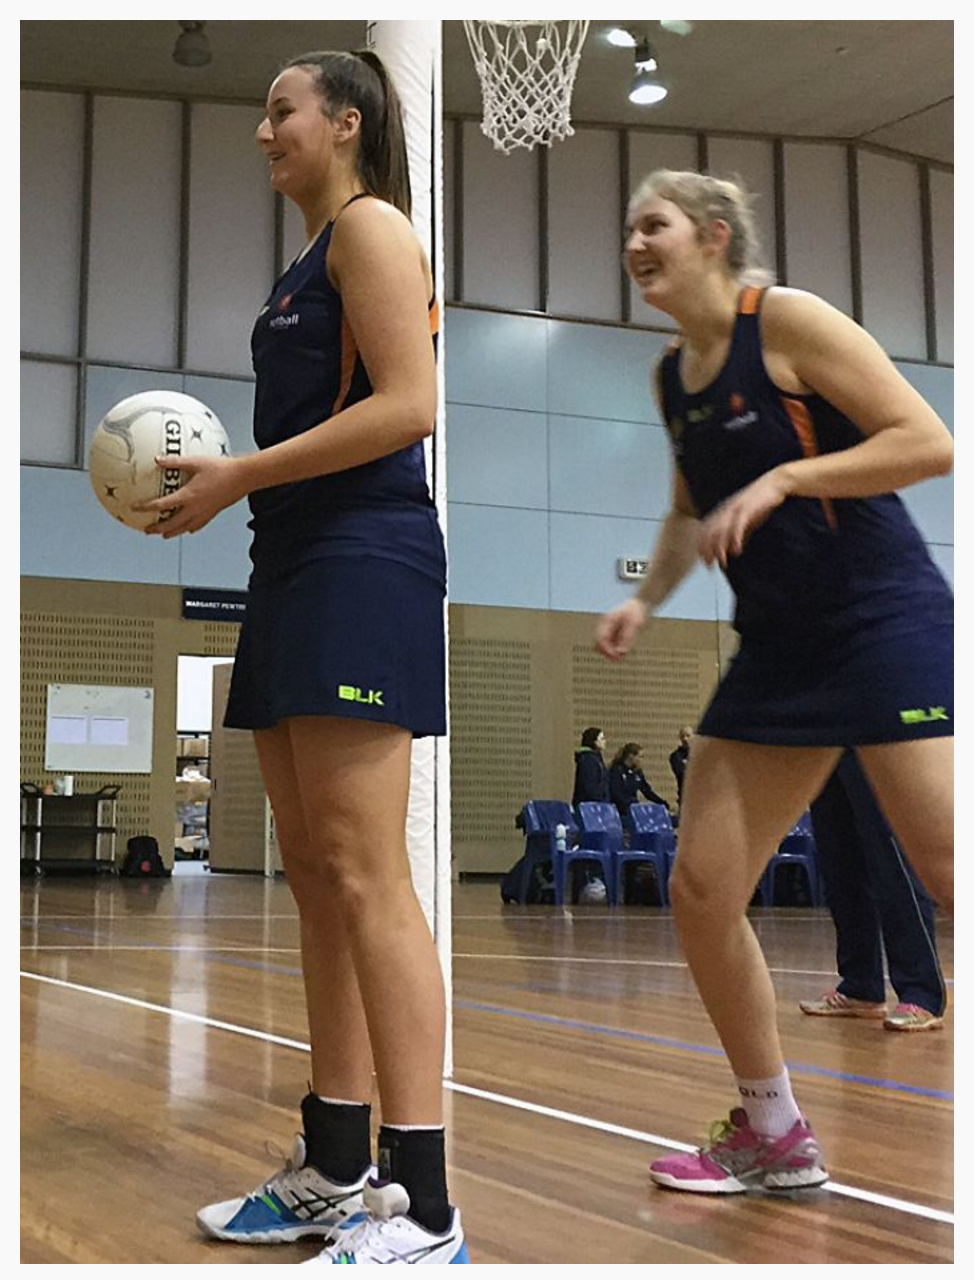
\includegraphics[height=6cm]{../images/NetballHeight.jpg}
\end{center}

\end{frame}


\begin{frame}{}

If $X$ represents the heights of Australian women (in cms), what is $P(X > 189)$?

\vspace{1cm}
\begin{knitrout}
\definecolor{shadecolor}{rgb}{0.969, 0.969, 0.969}\color{fgcolor}
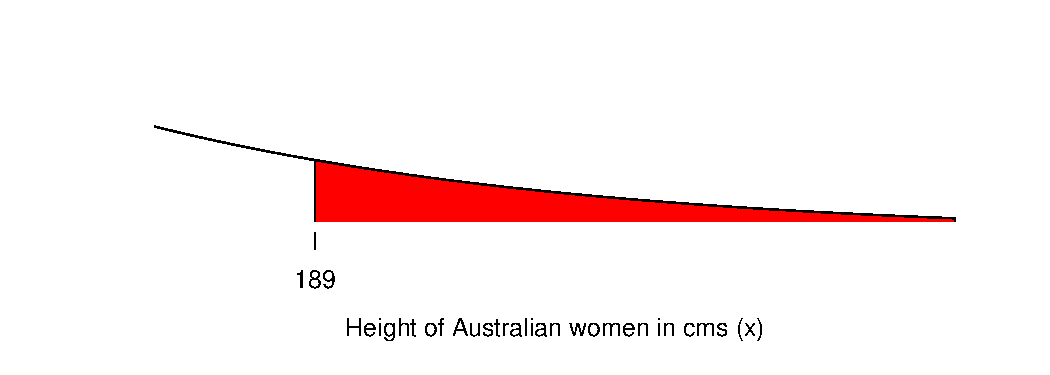
\includegraphics[width=\maxwidth]{figure/unnamed-chunk-2-1} 

\end{knitrout}
\end{frame}



\begin{frame}[fragile]{}

Similarly, in the Australian Football League (AFL) recruiters tend to look for tall male players.

\vspace{.5cm}
'Data collected by Adelaide sports doctor Geoffrey Verrall and AFL sports scientist Jamie Hepner suggest genetics play a bigger part in achieving a top-level football career than skill or desire. Using AFL statistics, they noted the height of the 562 rookies selected in AFL national drafts between 2004 and 2010. They found those shorter than 180cm could just about forget trying for a place in the elite league - unless they happened to be an indigenous or Pacific Islander player, who thrive on leg speed and lightning reflexes ... Generally, white Australian males must be tall (about 188cm) to  make it in the AFL.'
\href{http://www.heraldsun.com.au/sport/afl/size-matters-at-afl-level/story-e6frf9jf-1226650225771}{\beamergotobutton{HeraldSun}}
\end{frame}


\begin{frame}{}

{\bf What proportion of Australian men are similar height to Sydney superstar Adam Goodes (191cm) or West Coast ruckman Nick Naitanui (201cm)?}

\begin{center}
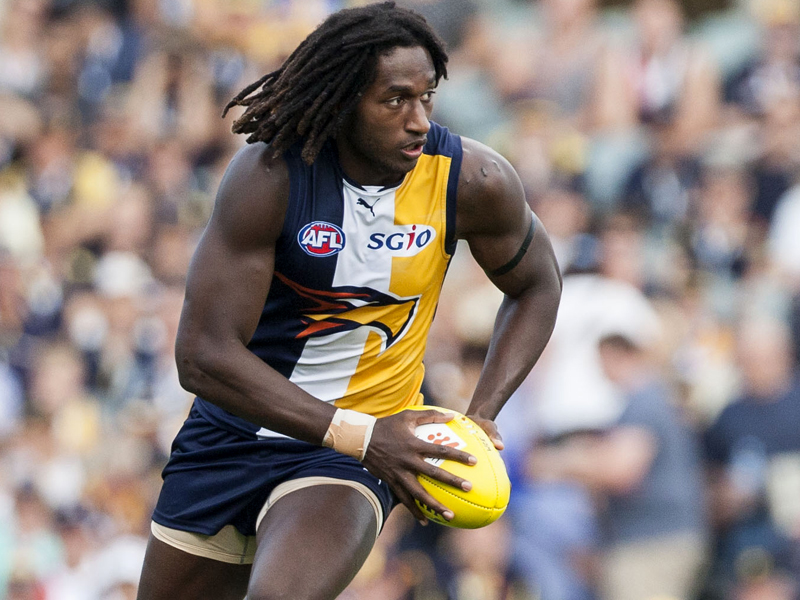
\includegraphics[height=6cm]{../images/NicN.jpg}
\end{center}

\href{http://www.sbs.com.au/news/sites/sbs.com.au.news/files/images/1/5/15Apr_NicNaitanui_800x600.jpg}{\beamergotobutton{SBS}}
\end{frame}


\begin{frame}{}

If $Y$ represents the heights of Australian men (in cms), what is $P(Y > 191)$ or even $P(Y > 201)$?

\vspace{1cm}
\begin{knitrout}
\definecolor{shadecolor}{rgb}{0.969, 0.969, 0.969}\color{fgcolor}
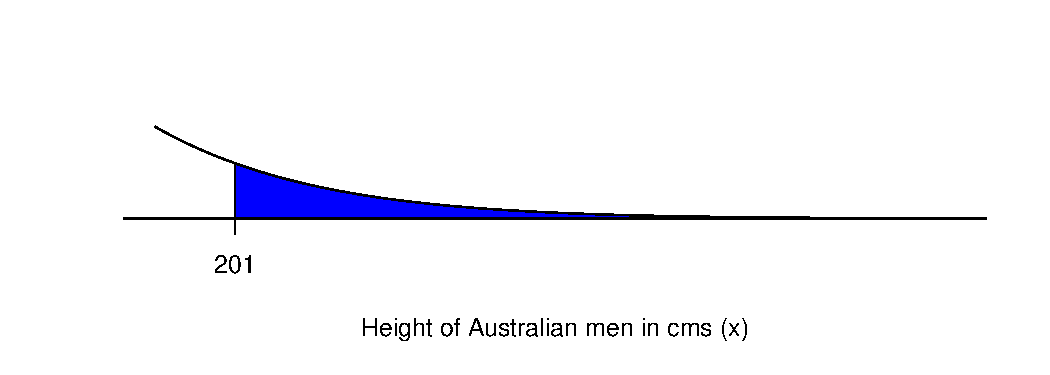
\includegraphics[width=\maxwidth]{figure/unnamed-chunk-3-1} 

\end{knitrout}
\end{frame}


\subsection[Comparing Discrete and Continuous Distributions]{Comparing Discrete and Continuous Distributions}
\begin{frame}\frametitle{Comparing Discrete and Continuous Distributions}

There are 5 fundamental differences between discrete and continuous distributions:

\vspace{.5cm}
\begin{tabular}{|l||l|l|} \hline 
 & Discrete & Continuous \\ \hline \hline
Values & Countable & Infinite \\ \hline
Plot &  Histogram $P(X=x)$ & Smooth curve $f(x)$  \\ 
& probability distribution & probability density \\
& function  & function (pdf)  \\ \hline
$P(X=x)$ & $0 \leq P(X=x) \leq 1 \;\; \forall x$
& $P(X=x)=0 \;\; \forall x$ \\ \hline
Sum of & $\sum_{x} P(X=x) = 1$ & $\int_{x} f(x) dx = 1$ \\
Probabilities & Area of histogram & Area under density \\ \hline
$F(x) = P(X \leq x)$ & $\sum_{y=min(x)}^{x} P(X=y)$
& $\int_{-\infty}^{x} f(y) dy$\\
CDF 
\hyperlink{CDF}{\beamergotobutton{CDF}}
& & \\ \hline
\end{tabular}

%Define CDF.
\end{frame}

\begin{frame}\frametitle{}

For any continuous distribution:

\begin{itemize}
\item
there is an infinite number of possible values;
\item
these values may be within a fixed interval. For example, male human heights (in cm) belong to [54.6,272].
\hyperlink{https://en.wikipedia.org/wiki/Human_height}{\beamergotobutton{Human Heights}}
\item
each of the individual probabilities is 0, ie $P(X=x)=0 \;\; \forall x$. This looks strange at first. However, consider that if we allocate even the smallest amount of probability to each of the infinite values, the probabilities could never sum to 1!
\item
the total of all the probabilites, represented by the area under the probability density function (pdf), must be  1.
\item For a continuous distribution
\[ P(a < X < b) = P(a \leq X \leq b) \] 
This is not generally true for a discrete distribution.
\end{itemize}
\end{frame}


\subsection[Normal Distribution]{Normal Distribution}

\begin{frame}[fragile,label=Normalpdf]\frametitle{Normal Distribution}

\begin{definition}[Normal Distribution]
The \alert{Normal distribution} models a symmetric, bell-shaped variable with 2 parameters mean $\mu$ and variance $\sigma^2$ and points of inflection at $\mu \pm \sigma$. We say the variable $X \sim N(\mu, \sigma^2)$. 

\vspace{.5cm}
The probability density function (pdf) is:
\[ f(x)  =  \frac{1}{  \sqrt{2 \pi \sigma^2}}  e^{   -\frac{ (x-\mu)^2 }{2 \sigma^2  } }
\;\;\;\;\; \mbox{for }  x \in (- \infty, \infty) \]

The cumulative distribution function (CDF) is
\[ F(x) = P(X \leq x) = \int_{-\infty}^{x} f(y) dy \]
\end{definition}

\end{frame}


\begin{frame}[fragile]\frametitle{}

The Normal Distribution is very important because it can approximate many natural phenomemon, like annual rainful (sometimes skewed), humidity, evapotranspiration, heights/weights/length of animals, intelligence, and measurement errors. \\

\vspace{.5cm}
It can also approximate sums of random variables, via the Central Limit Theorem (Topic 7). \\

\vspace{.5cm}
{\bf Does the Normal Distribution approximate the distribution of human heights?}

\end{frame}






\begin{frame}[fragile]

\href{http://www.abs.gov.au/websitedbs/CaSHome.nsf/Home/CensusAtSchool+data+for+Calculators#2012}{\beamergotobutton{Data}}


\begin{knitrout}
\definecolor{shadecolor}{rgb}{0.969, 0.969, 0.969}\color{fgcolor}\begin{kframe}
\begin{alltt}
\hlcom{## data <- read.csv("SchoolCensusHeights.csv")}
\hlkwd{names}\hlstd{(data)}
\end{alltt}
\begin{verbatim}
## [1] "FemaleHeight" "MaleHeight"   "AllHeight"
\end{verbatim}
\begin{alltt}
\hlkwd{par}\hlstd{(}\hlkwc{mfrow}\hlstd{=}\hlkwd{c}\hlstd{(}\hlnum{1}\hlstd{,}\hlnum{3}\hlstd{))}
\hlkwd{hist}\hlstd{(data}\hlopt{$}\hlstd{FemaleHeight)}
\hlkwd{hist}\hlstd{(data}\hlopt{$}\hlstd{MaleHeight)}
\hlkwd{hist}\hlstd{(data}\hlopt{$}\hlstd{AllHeight)}
\end{alltt}
\end{kframe}
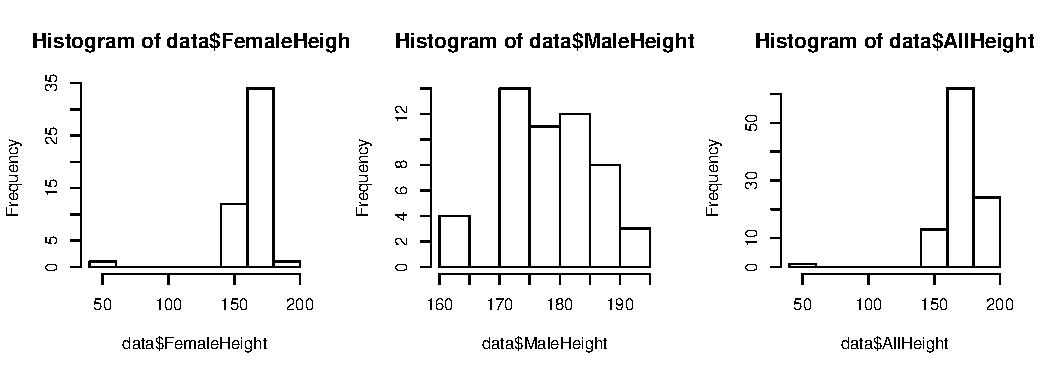
\includegraphics[width=\maxwidth]{figure/unnamed-chunk-4-1} 

\end{knitrout}

\end{frame}

\begin{frame}[fragile]

\href{https://vincentarelbundock.github.io/Rdatasets/doc/car/Davis.html}{\beamergotobutton{Data}}

\begin{knitrout}
\definecolor{shadecolor}{rgb}{0.969, 0.969, 0.969}\color{fgcolor}\begin{kframe}
\begin{alltt}
\hlcom{## data <- read.csv("DavisHeights.csv")}
\hlkwd{names}\hlstd{(data)}
\end{alltt}
\begin{verbatim}
## [1] "FemaleWeight" "MaleWeight"   "FemaleHeight" "MaleHeight"  
## [5] "ReportFW"     "ReportMW"     "ReportFH"     "ReportMH"
\end{verbatim}
\begin{alltt}
\hlkwd{par}\hlstd{(}\hlkwc{mfrow}\hlstd{=}\hlkwd{c}\hlstd{(}\hlnum{1}\hlstd{,}\hlnum{2}\hlstd{))}
\hlkwd{hist}\hlstd{(data}\hlopt{$}\hlstd{FemaleHeight)}
\hlkwd{hist}\hlstd{(data}\hlopt{$}\hlstd{ReportFH)}
\end{alltt}
\end{kframe}
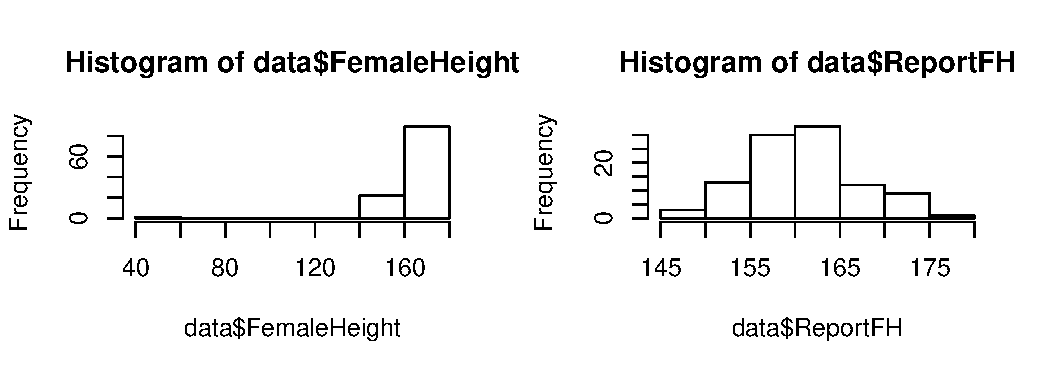
\includegraphics[width=\maxwidth]{figure/unnamed-chunk-5-1} 

\end{knitrout}
\end{frame}






\begin{frame}[fragile]

Modelling Australian women's heights by $X \sim N(161.8,6^2)$ and men by $Y \sim N(175.6,7^2)$, we get \\
\href{http://www.abs.gov.au/ausstats/abs@.nsf/0/E11CED5FB86D178ACA257AA30014C059?opendocument
}{\beamergotobutton{ABSData}}


\begin{knitrout}
\definecolor{shadecolor}{rgb}{0.969, 0.969, 0.969}\color{fgcolor}
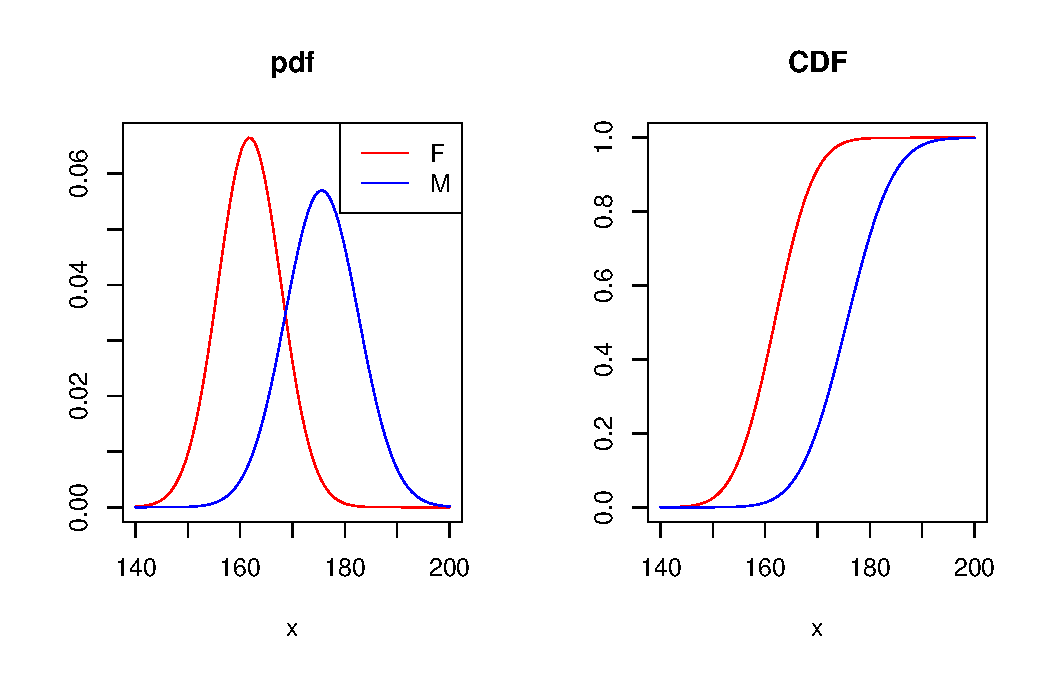
\includegraphics[width=\maxwidth]{figure/unnamed-chunk-7-1} 

\end{knitrout}
\end{frame}


\subsection[Normal Probabilities]{Normal Probabilities}

\begin{frame}[fragile]\frametitle{Normal Probabilities}

{\bf What is the probability of finding an Australian woman of `goal player' height or taller?} \\

\vspace{.5cm}
If $X \sim N(161.8,6^2)$, what is $P(X > 189)$?


\vspace{1cm}
\begin{knitrout}
\definecolor{shadecolor}{rgb}{0.969, 0.969, 0.969}\color{fgcolor}
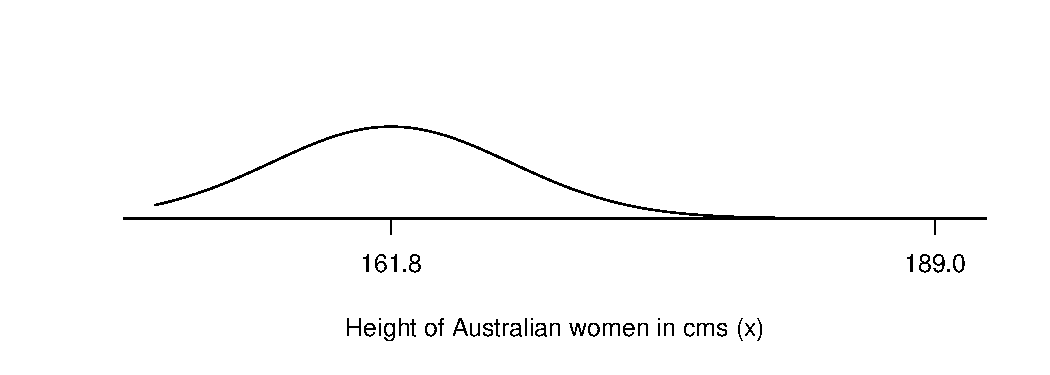
\includegraphics[width=\maxwidth]{figure/unnamed-chunk-8-1} 

\end{knitrout}
\end{frame}


\begin{frame}[fragile]\frametitle{}
{\bf Method1: Integrate the pdf} \\

\[ P(X > 189) = \int_{189}^{\infty} \frac{1}{  \sqrt{2 \pi (6^2)}}  e^{   -\frac{ (y-161.8)^2 }{2 (6^2)  } } dy \]


\vspace{1cm}
There is no closed form, but we could Numerical Integration.
\begin{knitrout}
\definecolor{shadecolor}{rgb}{0.969, 0.969, 0.969}\color{fgcolor}\begin{kframe}
\begin{alltt}
\hlstd{f} \hlkwb{<-} \hlkwa{function}\hlstd{(}\hlkwc{x}\hlstd{) \{}\hlkwd{dnorm}\hlstd{(x,}\hlnum{161.8}\hlstd{,}\hlnum{6}\hlstd{)\}}
\hlkwd{integrate}\hlstd{(f,}\hlnum{189}\hlstd{,}\hlnum{200}\hlstd{)}
\end{alltt}
\begin{verbatim}
## 2.902907e-06 with absolute error < 3.2e-20
\end{verbatim}
\end{kframe}
\end{knitrout}
\end{frame}


\begin{frame}[fragile]\frametitle{}

{\bf Method2: Use R}

\begin{knitrout}
\definecolor{shadecolor}{rgb}{0.969, 0.969, 0.969}\color{fgcolor}\begin{kframe}
\begin{alltt}
\hlkwd{pnorm}\hlstd{(}\hlnum{189}\hlstd{,}\hlnum{161.8}\hlstd{,}\hlnum{6}\hlstd{)}  \hlcom{#pnorm(x,mean,sd) }
\end{alltt}
\begin{verbatim}
## [1] 0.9999971
\end{verbatim}
\end{kframe}
\end{knitrout}

\begin{knitrout}
\definecolor{shadecolor}{rgb}{0.969, 0.969, 0.969}\color{fgcolor}
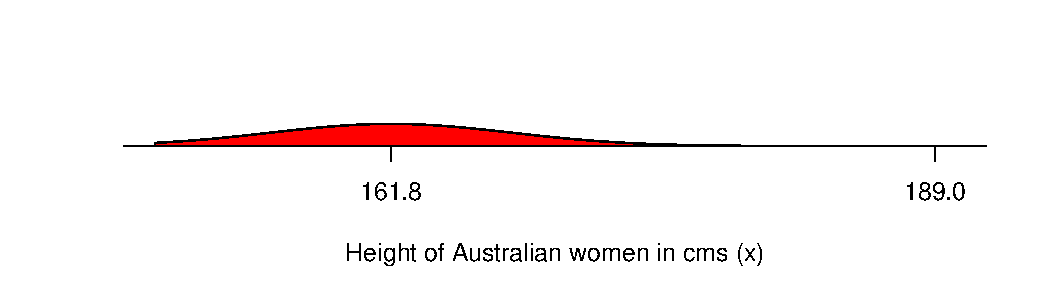
\includegraphics[width=\maxwidth]{figure/unnamed-chunk-11-1} 

\end{knitrout}

Upper Tail probabilities are found from Lower Tail probabilties:
\[ P(X > 189) = 1- P(X \leq 189) = 2.9e-06 \]

\end{frame}




\begin{frame}[fragile]
Notes on using R:
\begin{itemize}
\item
Interval probabilities are found by subtraction:
\[ P( 170 < X \leq 175) = 0.07196146 \]

\begin{knitrout}
\definecolor{shadecolor}{rgb}{0.969, 0.969, 0.969}\color{fgcolor}
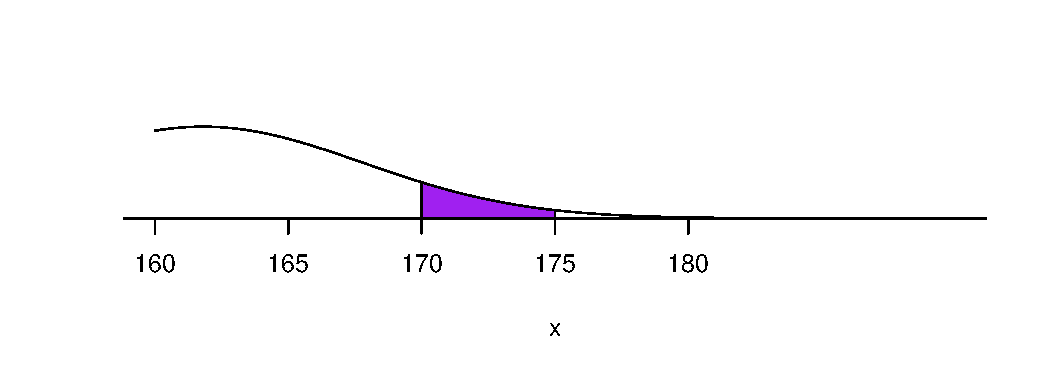
\includegraphics[width=\maxwidth]{figure/unnamed-chunk-12-1} 

\end{knitrout}

\begin{knitrout}
\definecolor{shadecolor}{rgb}{0.969, 0.969, 0.969}\color{fgcolor}\begin{kframe}
\begin{alltt}
\hlkwd{pnorm}\hlstd{(}\hlnum{175}\hlstd{,}\hlnum{161.8}\hlstd{,}\hlnum{6}\hlstd{)}\hlopt{-}\hlkwd{pnorm}\hlstd{(}\hlnum{170}\hlstd{,}\hlnum{161.8}\hlstd{,}\hlnum{6}\hlstd{)}
\end{alltt}
\begin{verbatim}
## [1] 0.07196146
\end{verbatim}
\end{kframe}
\end{knitrout}
\end{itemize}
\end{frame}

\begin{frame}[fragile]
\begin{itemize}
\item
For the standard Normal $Z \sim N(0,1)$, we can leave the mean and standard deviation unspecified.

\[ P(Z \leq 0.8)  = 0.7881446 \]

\begin{knitrout}
\definecolor{shadecolor}{rgb}{0.969, 0.969, 0.969}\color{fgcolor}
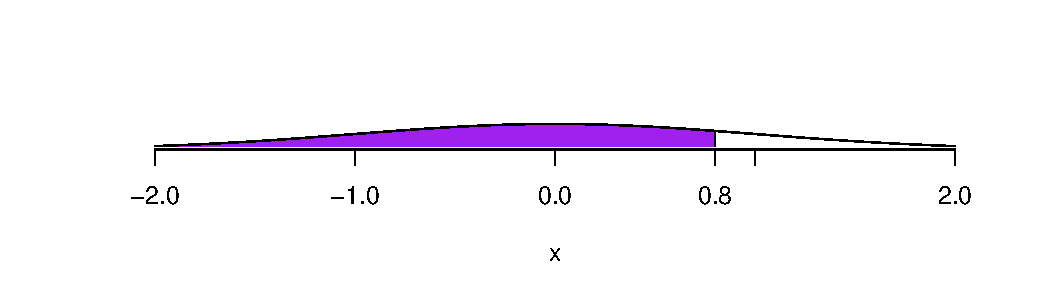
\includegraphics[width=\maxwidth]{figure/unnamed-chunk-14-1} 

\end{knitrout}

\begin{knitrout}
\definecolor{shadecolor}{rgb}{0.969, 0.969, 0.969}\color{fgcolor}\begin{kframe}
\begin{alltt}
\hlkwd{pnorm}\hlstd{(}\hlnum{0.8}\hlstd{,}\hlnum{0}\hlstd{,}\hlnum{1}\hlstd{)}
\end{alltt}
\begin{verbatim}
## [1] 0.7881446
\end{verbatim}
\begin{alltt}
\hlkwd{pnorm}\hlstd{(}\hlnum{0.8}\hlstd{)}
\end{alltt}
\begin{verbatim}
## [1] 0.7881446
\end{verbatim}
\end{kframe}
\end{knitrout}

\end{itemize}
\end{frame}


\begin{frame}[fragile]\frametitle{}

{\bf Method3: Standardise and use the Standard Normal Tables} 

\vspace{.5cm}
The Standard Normal Tables tabulate the CDF for $Z \sim N(0,1)$. \\

\vspace{.5cm}
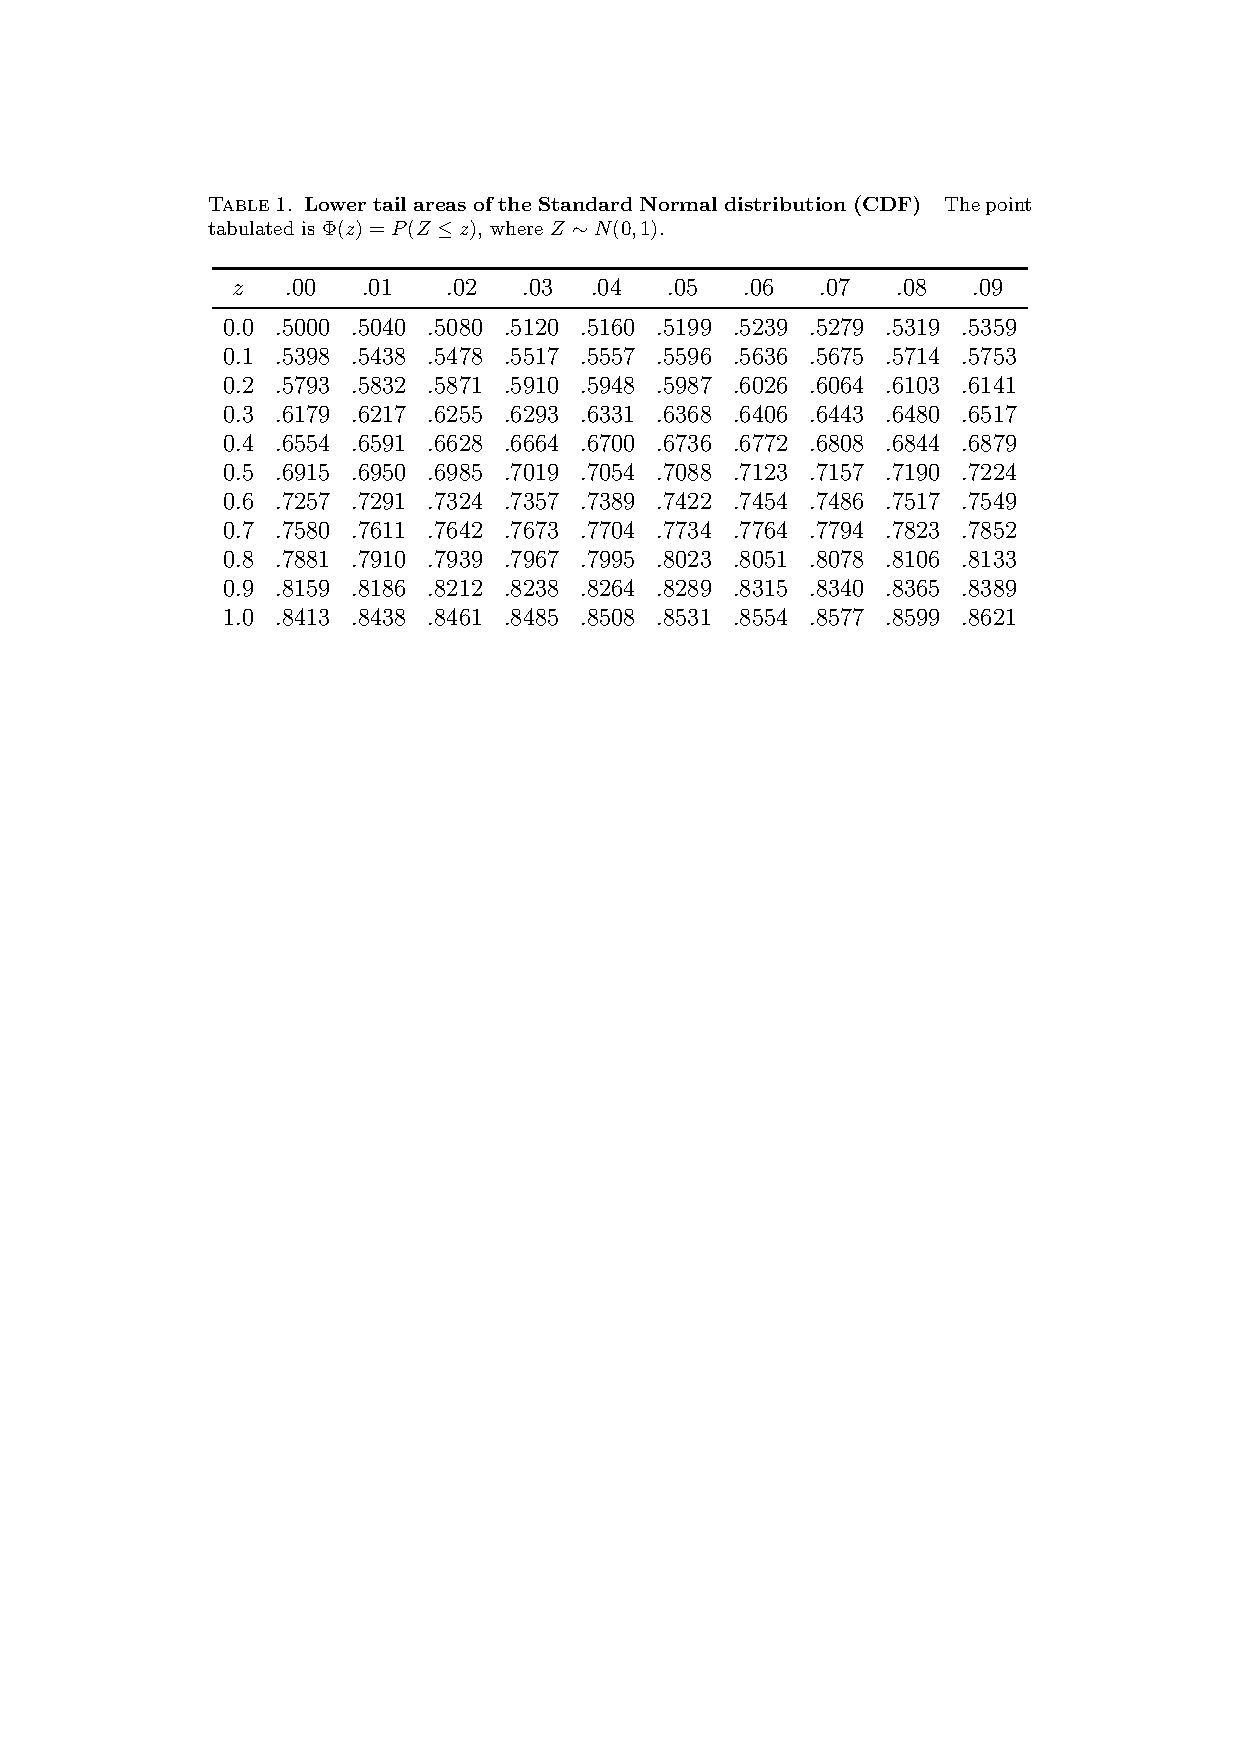
\includegraphics[height=6cm]{../images/NormalTableSample.pdf}

\end{frame}


\begin{frame}[fragile]\frametitle{}

For example, $P(Z \leq 0.8) = 0.7881$. \\

\begin{knitrout}
\definecolor{shadecolor}{rgb}{0.969, 0.969, 0.969}\color{fgcolor}
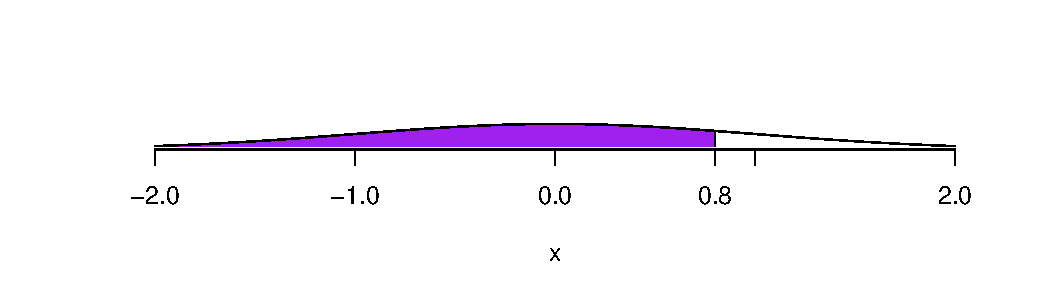
\includegraphics[width=\maxwidth]{figure/unnamed-chunk-16-1} 

\end{knitrout}

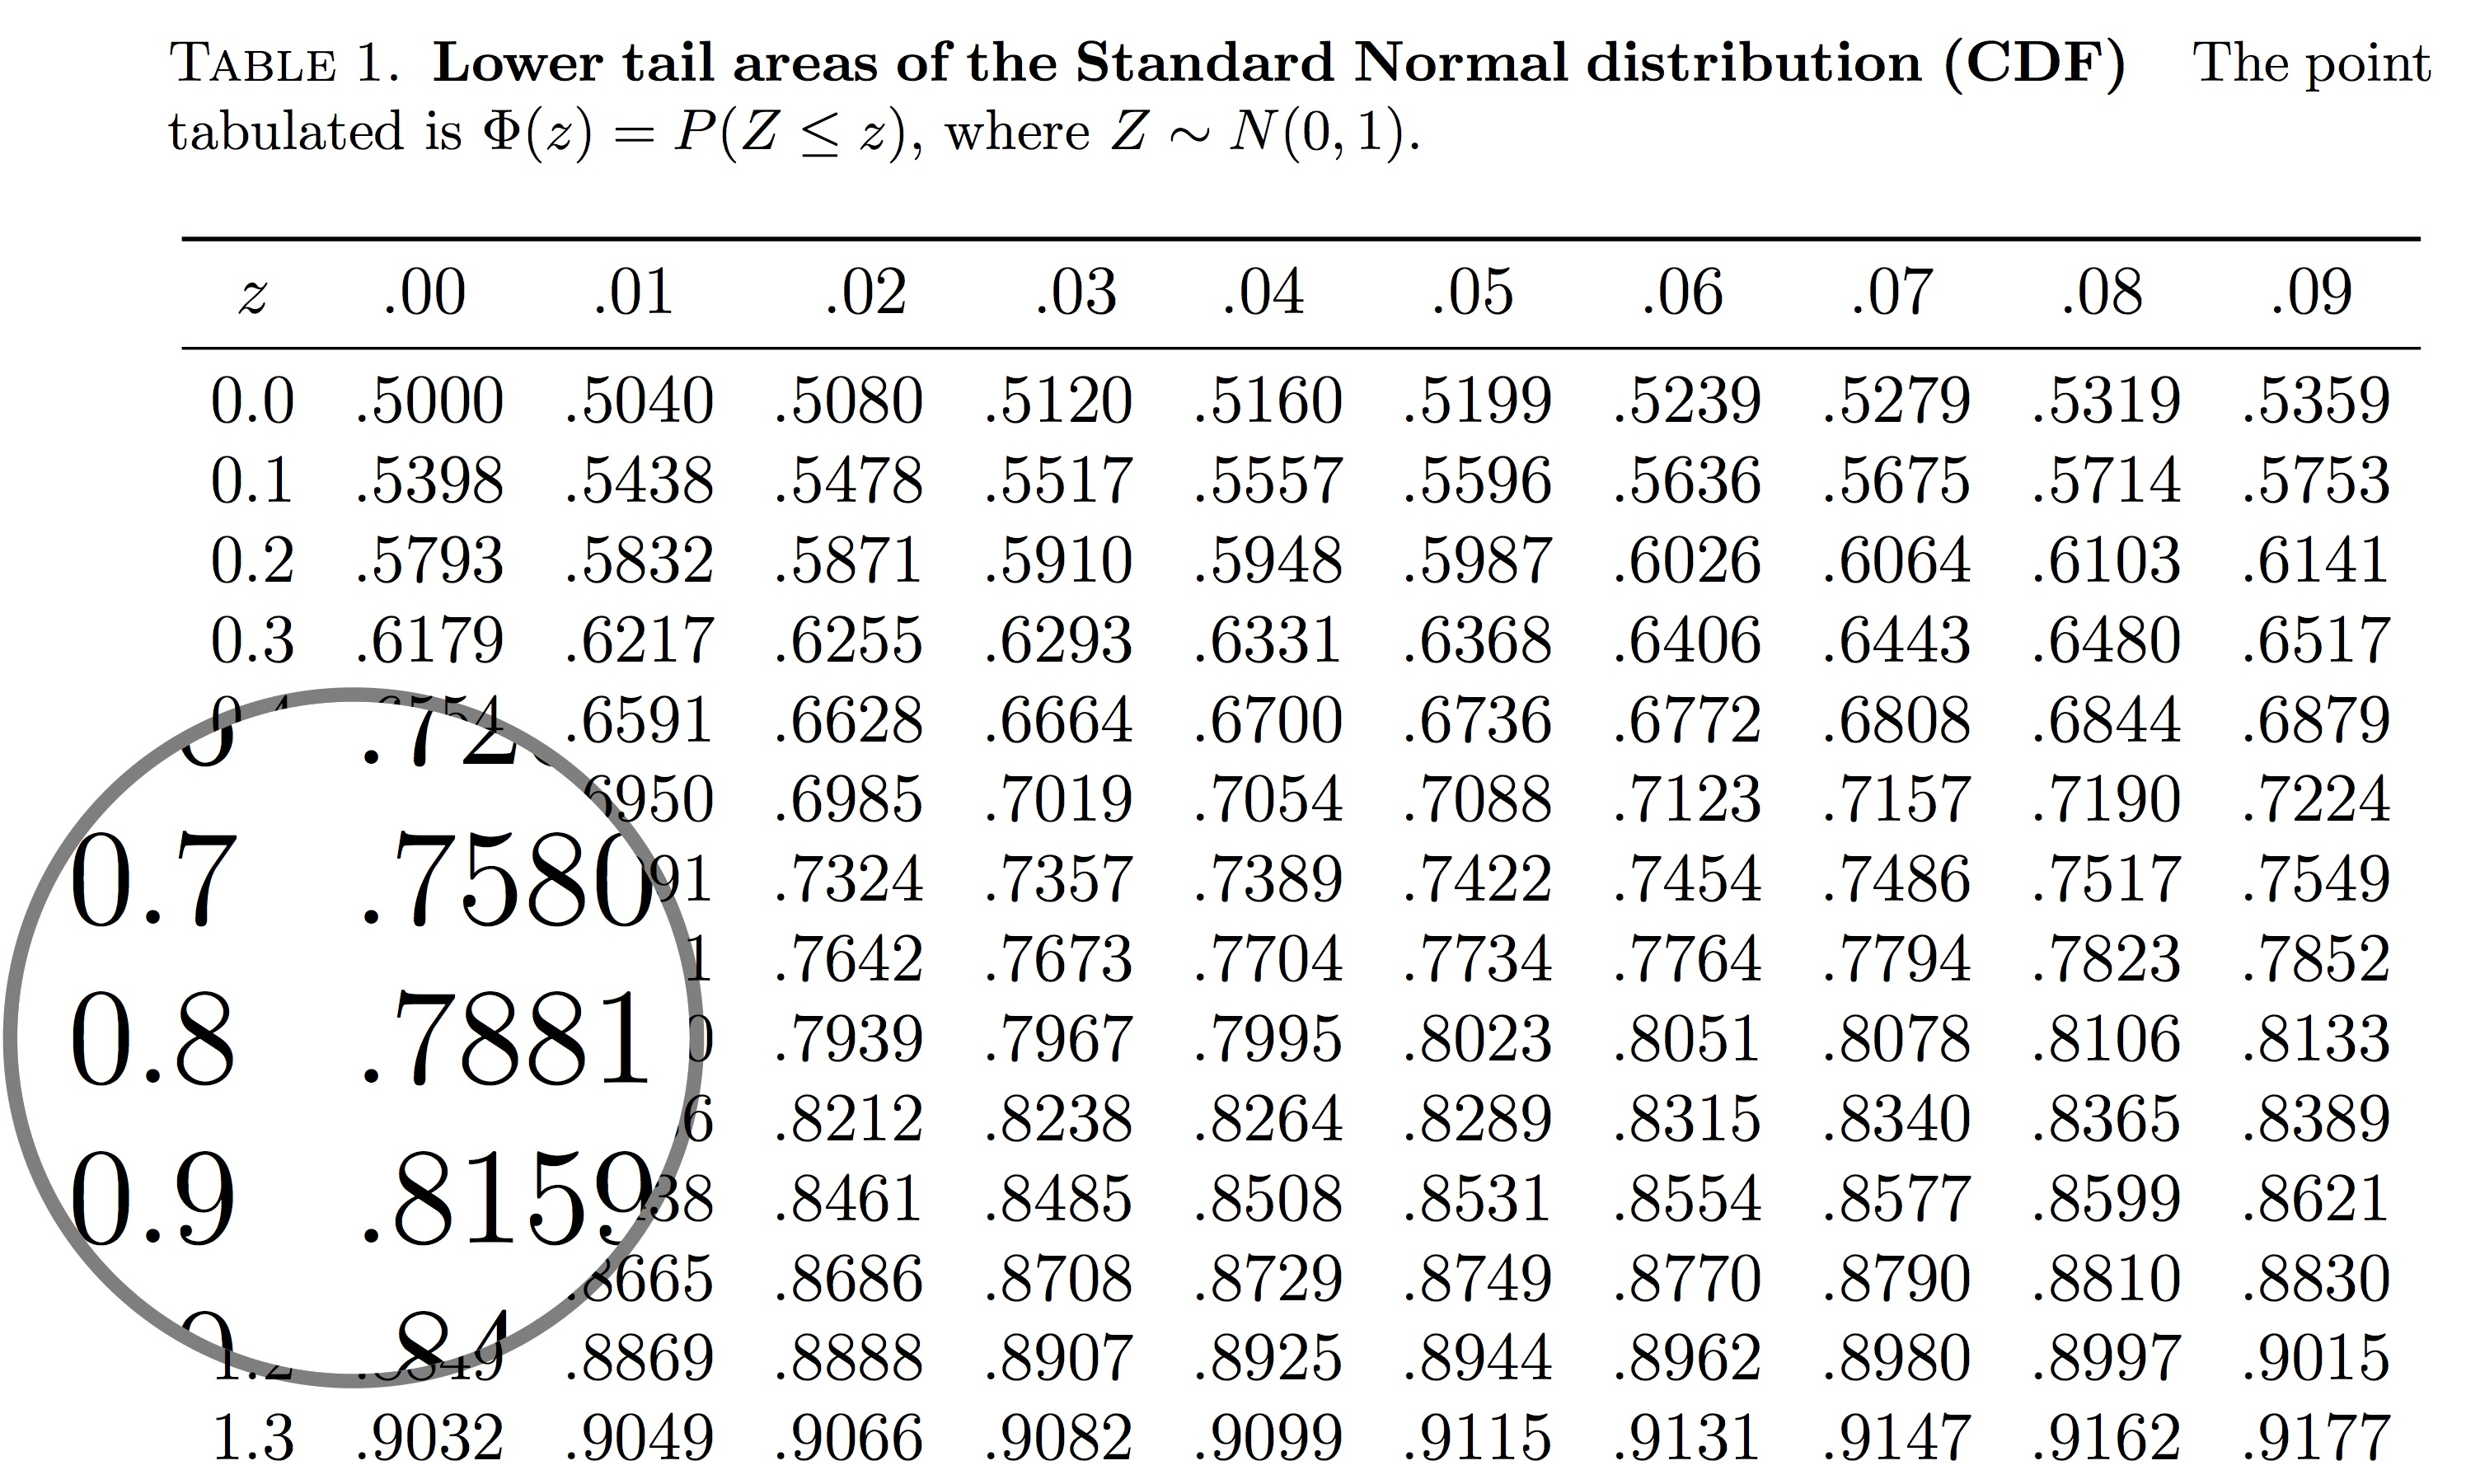
\includegraphics[height=5cm]{../images/NormalTableEg1.jpg}
\end{frame}

\begin{frame}\frametitle{}

How do we use the Standard Normal Tables for a general Normal?  \\ 

\vspace{.5cm} 
Every General Normal $X \sim N(\mu, \sigma^2)$ can be transformed into the Standard Normal $Z \sim N(0,1)$. 

\vspace{.5cm} 
\begin{definition}[Standardardising a Normal]
If $X \sim N(\mu, \sigma^2)$ and $Z \sim N(0, 1)$, then \\
$P( X \leq x) = P \Big( \frac{X-\mu}{\sigma} \leq \frac{x-\mu}{\sigma}  \Big)= P \Big( Z \leq \frac{x-\mu}{\sigma}  \Big)$
\end{definition}

\begin{eqnarray*}
P(X > 189) & = & P( \frac{X-161.8}{6} > \frac{189-161.8}{6}) \\
& = & P(Z > 4.533333)  \\
& < & 1-0.9986 \\
& = & 0.0014
\end{eqnarray*}
\end{frame}

\begin{frame}[fragile]\frametitle{}

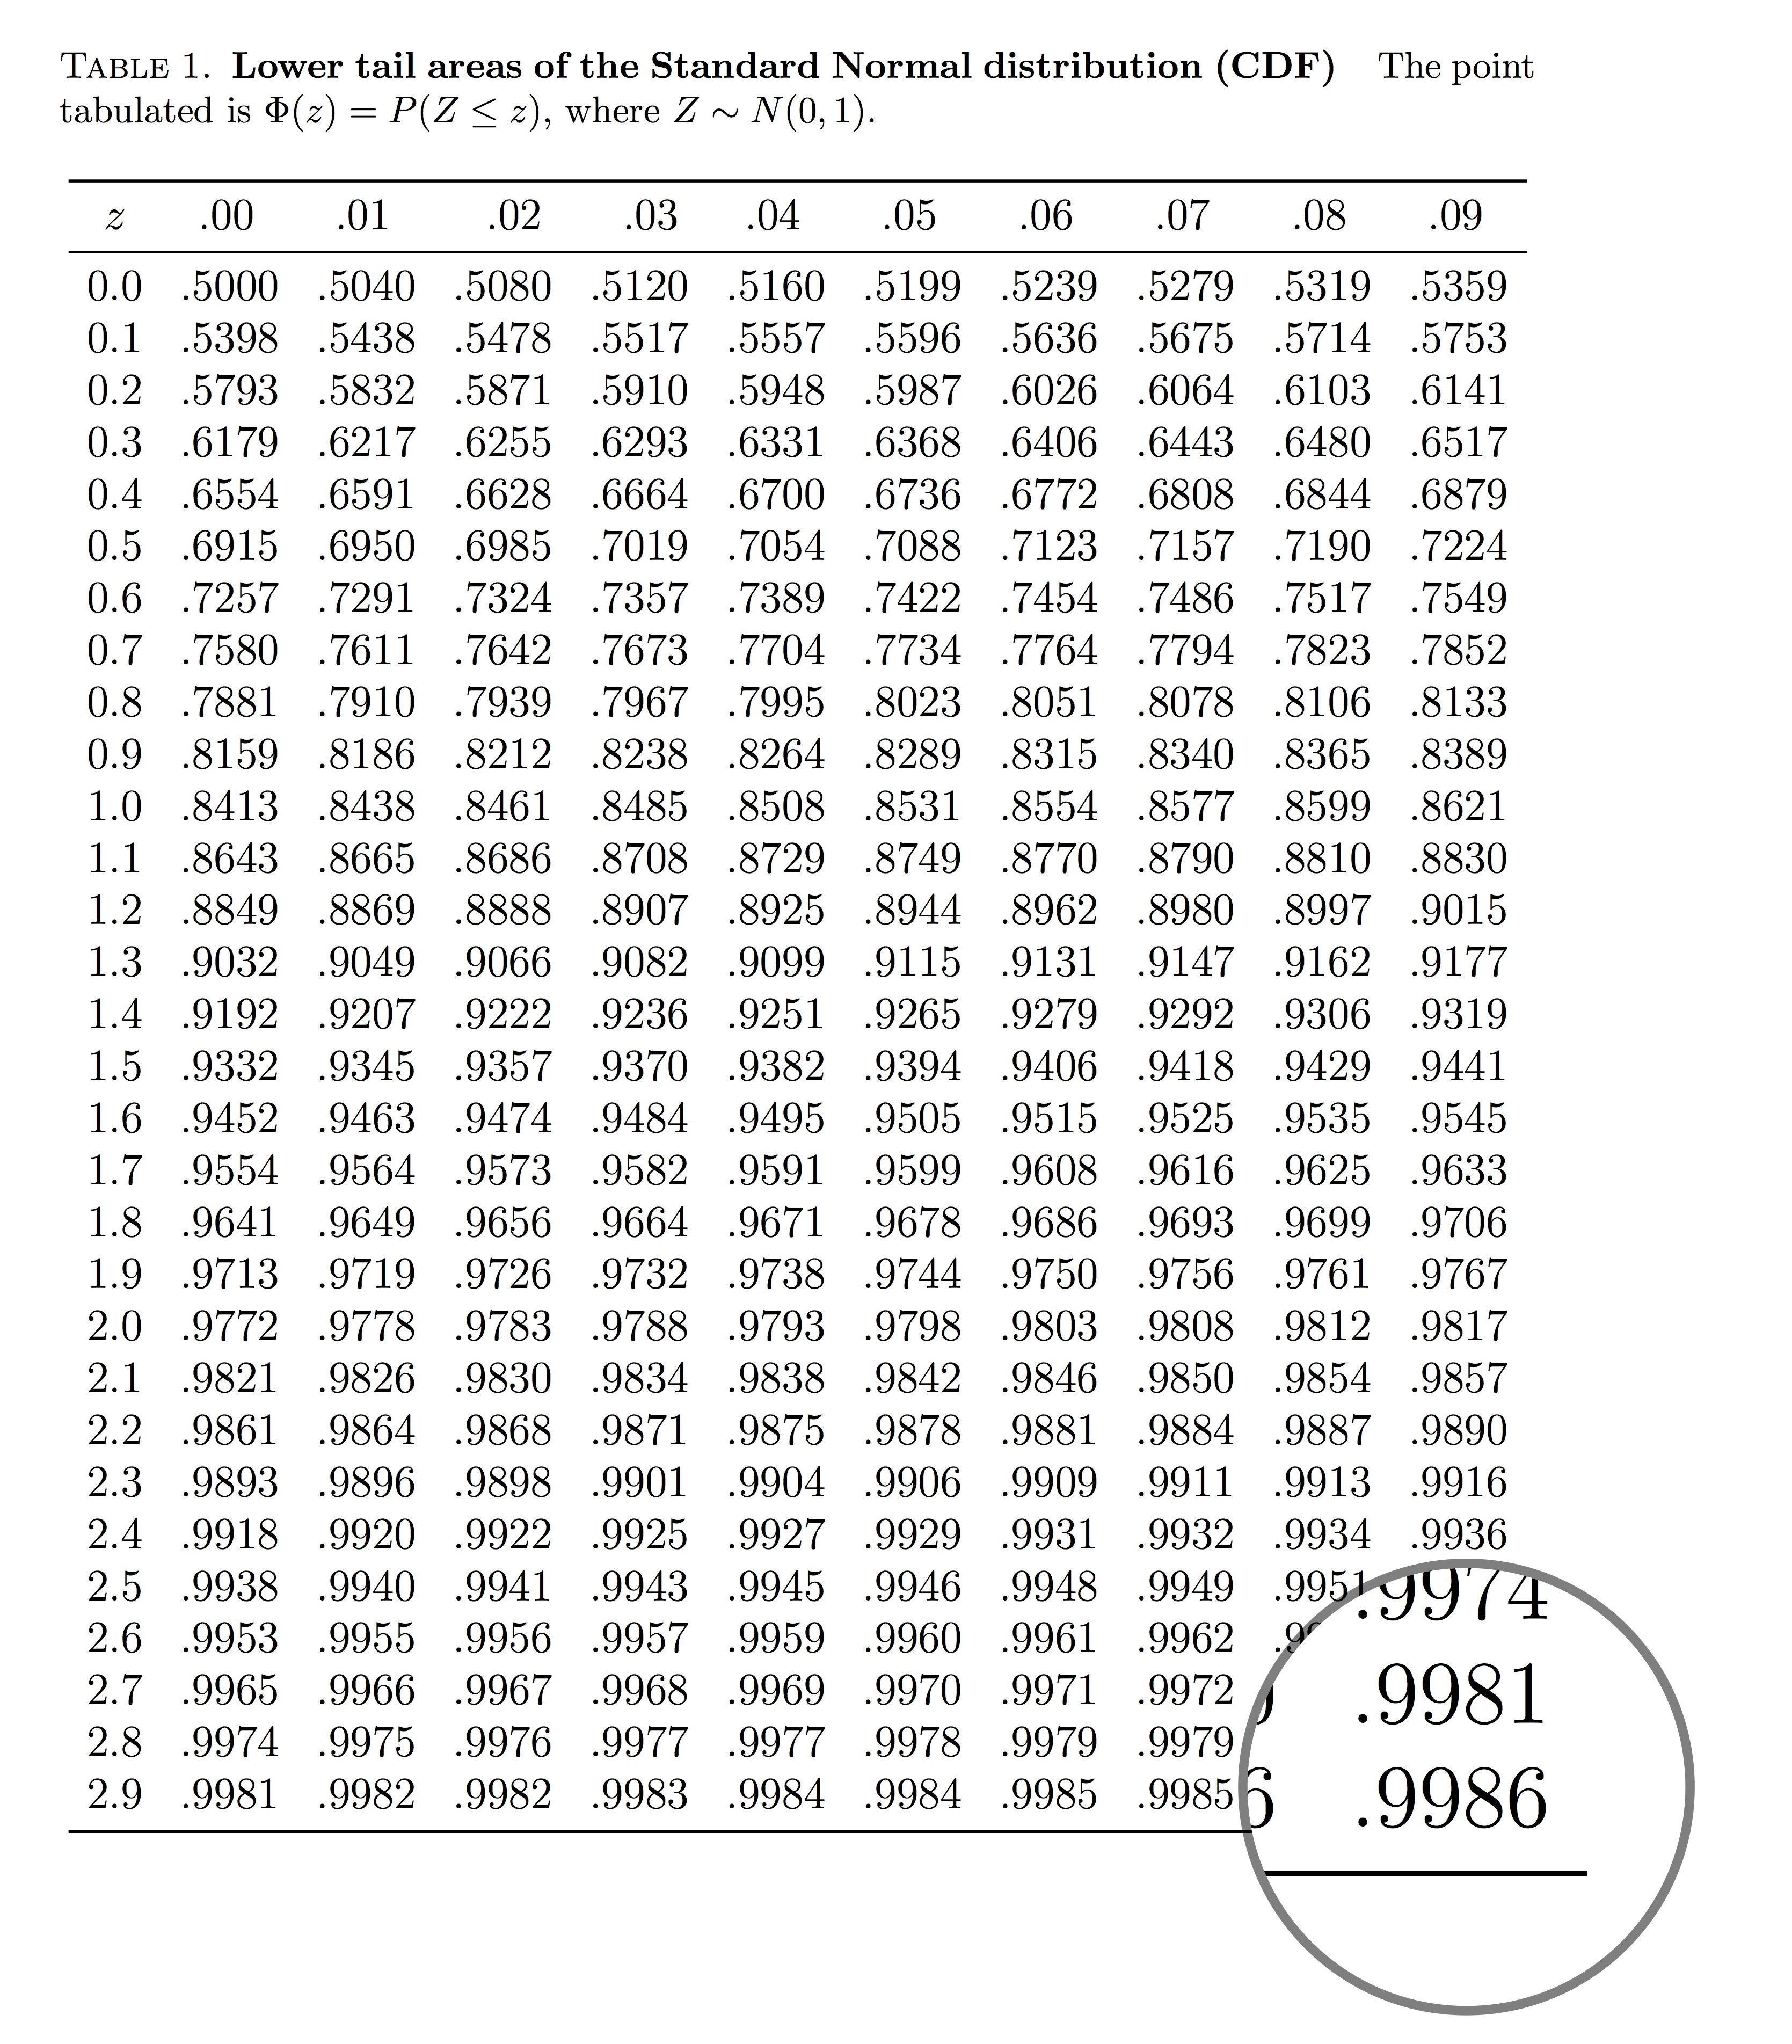
\includegraphics[height=8cm]{../images/NormalTableEg2.jpg}

\end{frame}


\begin{frame}[fragile]\frametitle{}

Effectively we have found that 
\begin{knitrout}
\definecolor{shadecolor}{rgb}{0.969, 0.969, 0.969}\color{fgcolor}
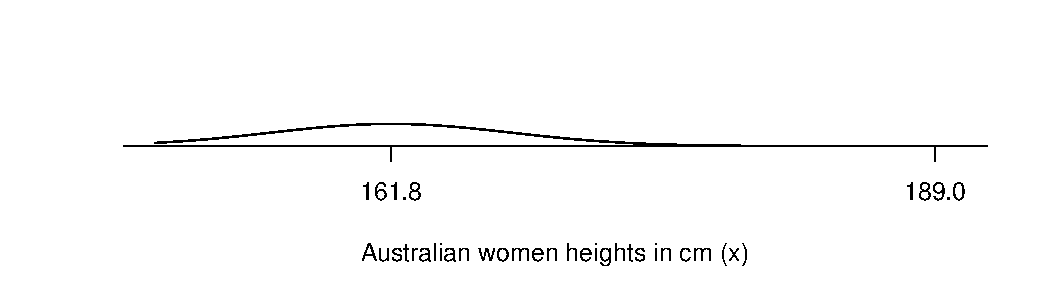
\includegraphics[width=\maxwidth]{figure/unnamed-chunk-17-1} 

\end{knitrout}
is equivalent to
\begin{knitrout}
\definecolor{shadecolor}{rgb}{0.969, 0.969, 0.969}\color{fgcolor}
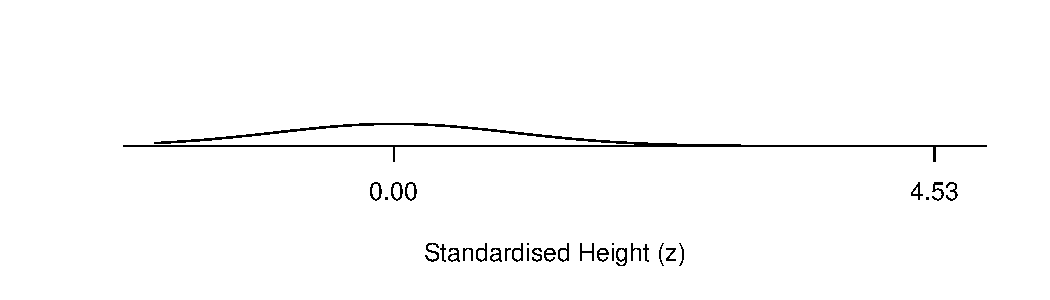
\includegraphics[width=\maxwidth]{figure/unnamed-chunk-18-1} 

\end{knitrout}

{\tiny
\begin{knitrout}
\definecolor{shadecolor}{rgb}{0.969, 0.969, 0.969}\color{fgcolor}\begin{kframe}
\begin{alltt}
\hlnum{1}\hlopt{-}\hlkwd{pnorm}\hlstd{(}\hlnum{4.533333}\hlstd{)}
\end{alltt}
\begin{verbatim}
## [1] 2.903009e-06
\end{verbatim}
\end{kframe}
\end{knitrout}
}
\end{frame}



\begin{frame}[fragile]\frametitle{}

{\bf Method4: Appoximate using the Special Percentiles of the Normal Distribution} 

All Normal distributions satisfy the "68\%-95\%-99.7\% Rule. \\

\vspace{.5cm}
\begin{tabular}{|l|l|} \hline
Number of sds $\sigma$ from the Mean $\mu$ & \% of Probability \\ \hline
1 & 68\%  \\
2 & 95\% \\
3 & 99.7\% \\ \hline
\end{tabular}


\begin{knitrout}
\definecolor{shadecolor}{rgb}{0.969, 0.969, 0.969}\color{fgcolor}
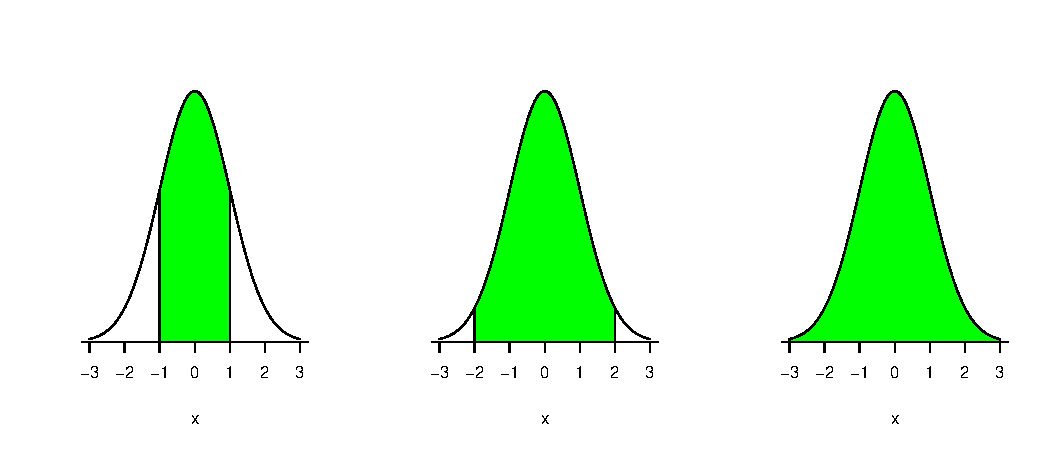
\includegraphics[width=\maxwidth]{figure/unnamed-chunk-20-1} 

\end{knitrout}

\end{frame}



\subsection[Normal Percentiles]{Normal Percentiles}
\begin{frame}[fragile]\frametitle{Normal Percentiles (Inverse Probabilities)}

Given $X \sim N(161.8,6^2)$, what is the 90\% percentile for heights of Australian women. \\

\vspace{.5cm}
We need to find $q$ such that $P(X \leq q) = 0.9$.

\begin{knitrout}
\definecolor{shadecolor}{rgb}{0.969, 0.969, 0.969}\color{fgcolor}
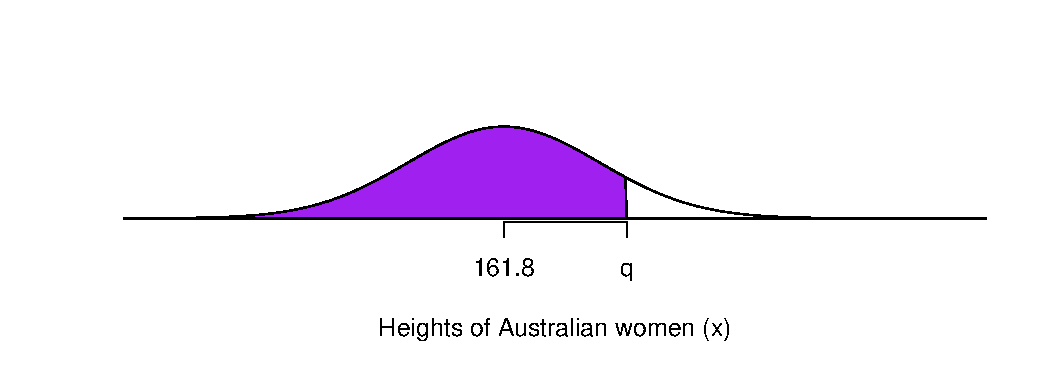
\includegraphics[width=\maxwidth]{figure/unnamed-chunk-21-1} 

\end{knitrout}

\begin{knitrout}
\definecolor{shadecolor}{rgb}{0.969, 0.969, 0.969}\color{fgcolor}\begin{kframe}
\begin{alltt}
\hlkwd{qnorm}\hlstd{(}\hlnum{0.9}\hlstd{,}\hlnum{161.8}\hlstd{,}\hlnum{6}\hlstd{)}  \hlcom{#qnorm(%,mean,sd)}
\end{alltt}
\begin{verbatim}
## [1] 169.4893
\end{verbatim}
\end{kframe}
\end{knitrout}
\end{frame}


\subsection[Other Distributions]{Other Continuous Distributions}


\begin{frame}\frametitle{Other Continuous Distributions}

We now consider 3 other continuous distributions which will be used in the Hypothesis Testing part of the course (Topic 8 onwards).

\begin{itemize}
\item Student $T$  (T tests)
\item Fisher's $F$ (Test for equal variance and ANOVA in STAT2)
\item Chi-Squared $\chi^{2}$ (Goodness of Fit Tests)
\end{itemize}

\end{frame}


\begin{frame}\frametitle{Student T}

\begin{definition}[Student T Distribution]
The \alert{Student T distribution} is symmetric and bell-shaped with thicker tails than a Normal. 

\vspace{.5cm}
We say the variable $X \sim t_{n}$, with $n$ degrees of freedom.

\vspace{.5cm}
The pdf is:
\[ f(x)  =  \frac{ \Gamma(\frac{n+1}{2})}  { \sqrt{n \pi} \Gamma(\frac{n}{2})}
(1+ \frac{x^2}{n})^{-\frac{n+1}{2}}
\;\;\;\;\; \mbox{for }  x \in (- \infty, \infty) \]
\hyperlink{Normalpdf}{\beamergotobutton{Compare Normal}} 

\vspace{.5cm}
The mean is 0 and variance is $\frac{n}{n-2}$ for $n > 2$.

\end{definition}
\end{frame}

\begin{frame}[fragile]\frametitle{}

\begin{knitrout}
\definecolor{shadecolor}{rgb}{0.969, 0.969, 0.969}\color{fgcolor}
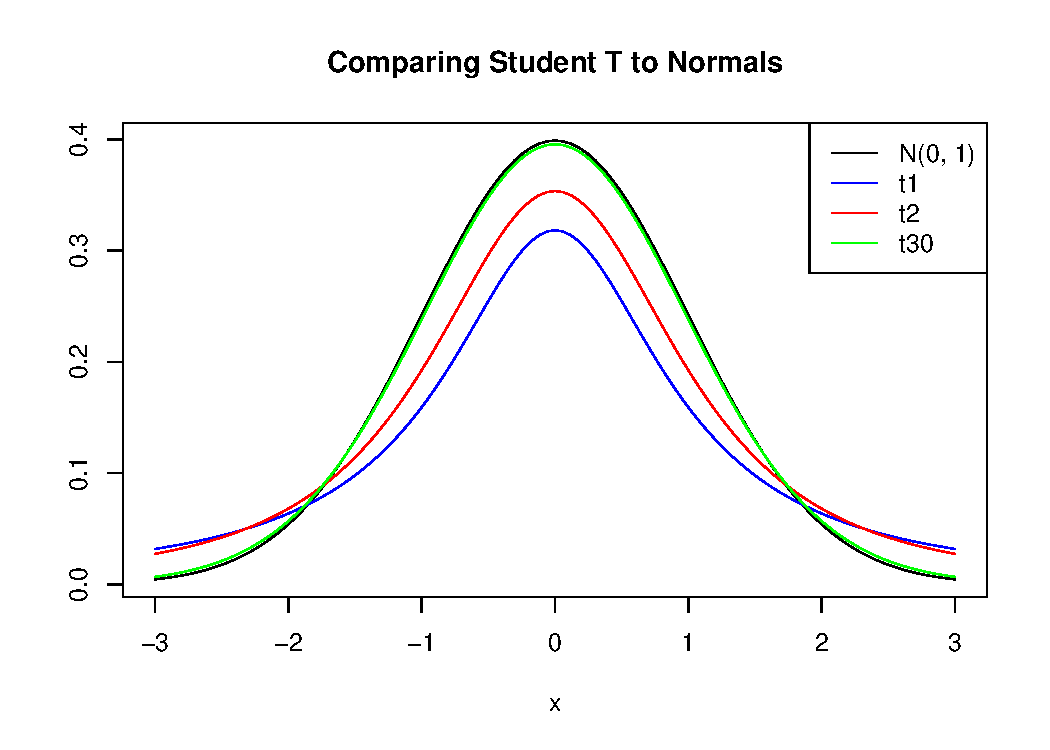
\includegraphics[width=\maxwidth]{figure/unnamed-chunk-23-1} 

\end{knitrout}
\end{frame}
 

\begin{frame}\frametitle{Chi-Squared distribution}

\vspace{.5cm}
\begin{definition}[Chi-Squared distribution]
The \alert{Chi-Squared distribution} is the sum of squared independent Standard Normal random variables. It can only take positive values and typically right skewed.

\vspace{.5cm}
We say the variable $X \sim \chi^2_{n}$, with $n$ degrees of freedom.

\vspace{.5cm}
The pdf is:
\[ f(x)  =  \frac{ 1}  { 2^{\frac{n}{2}} \Gamma(\frac{n}{2})}
x^{\frac{n}{2}-1} e^{-\frac{x}{2}}
\;\;\;\;\; \mbox{for }  x \in (0, \infty) \]

\vspace{.5cm}
The mean is $n$ and variance is $2 n$.
\end{definition}

\end{frame}



\begin{frame}[fragile]\frametitle{}
\begin{knitrout}
\definecolor{shadecolor}{rgb}{0.969, 0.969, 0.969}\color{fgcolor}
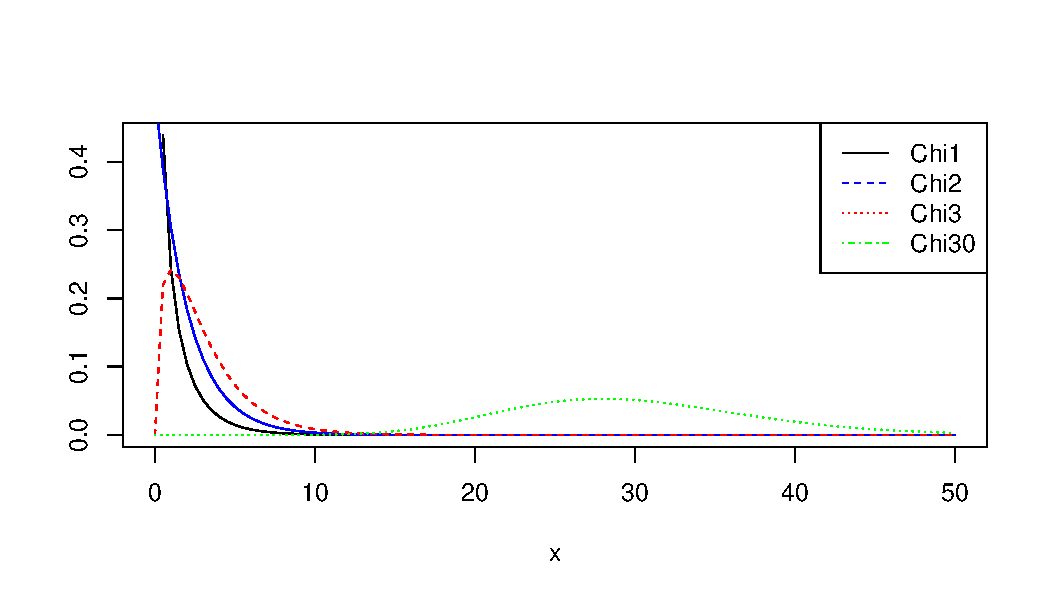
\includegraphics[width=\maxwidth]{figure/unnamed-chunk-24-1} 

\end{knitrout}

\end{frame}


\begin{frame}\frametitle{Fisher's F}

\begin{definition}[Fisher's F Distribution]
The \alert{Fisher's F distribution} is the scaled ratio of 2 $\chi^2$ variables, with $m$ and $n$ degrees of freedom.

\vspace{.5cm}
We say the variable $X \sim F_{m,n}$. \\

\vspace{.5cm}
The pdf is:
\[ f(x)  =  \frac{ \Gamma( \frac{m+n}{2} ) m^{\frac{m}{2}}  n^{\frac{n}{2}}   }{ \Gamma( \frac{m}{2} )  \Gamma( \frac{n}{2} )}
\frac{ x^{\frac{m}{2}-1}  }{ (n + mx)^{\frac{m+n}{2}}      }
\;\;\;\;\; \mbox{for }  x \in (0, \infty) \]



\vspace{.5cm}
The mean is $\frac{n}{n-2}$ for $n >2$ and variance is $\frac{2 n^2 (m+n-2)}{m (n-2)^2(n-4)}$ for $n > 4$.



\end{definition}

\end{frame}


\begin{frame}[fragile]\frametitle{}

\begin{knitrout}
\definecolor{shadecolor}{rgb}{0.969, 0.969, 0.969}\color{fgcolor}
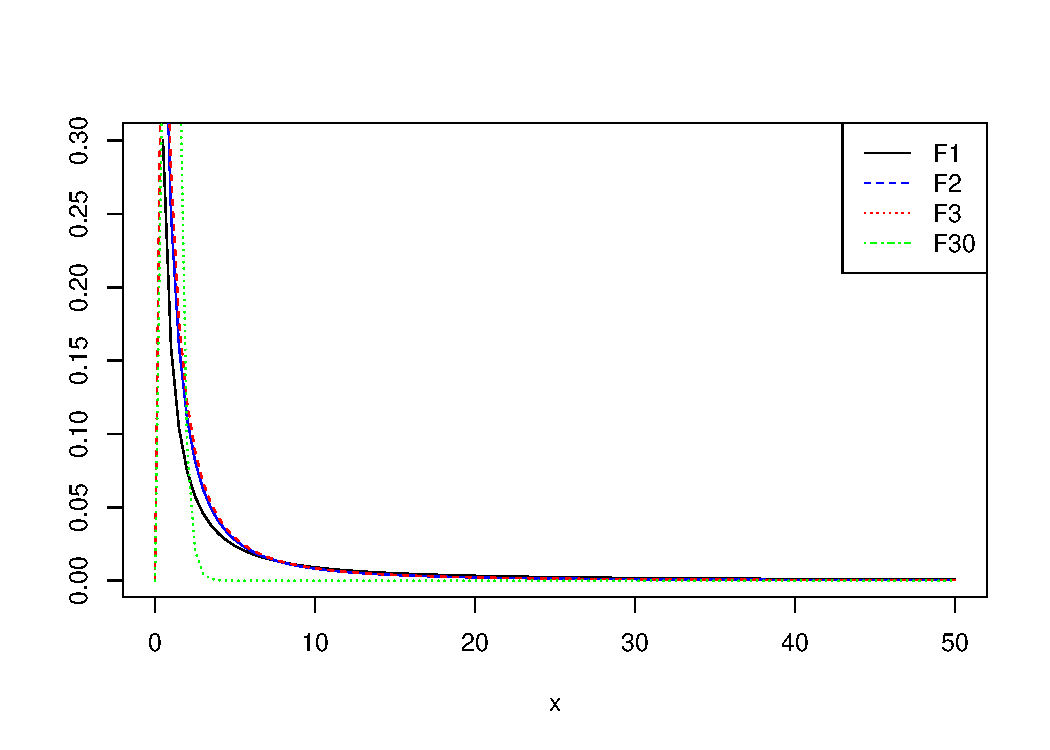
\includegraphics[width=\maxwidth]{figure/unnamed-chunk-25-1} 

\end{knitrout}
\end{frame}


\begin{frame}[fragile]\frametitle{}
 
Using commands in R: \\

$P(X \leq 2)$, where $X \sim t_{4}$.

\begin{knitrout}
\definecolor{shadecolor}{rgb}{0.969, 0.969, 0.969}\color{fgcolor}\begin{kframe}
\begin{alltt}
\hlkwd{pt}\hlstd{(}\hlnum{2}\hlstd{,}\hlnum{4}\hlstd{)}
\end{alltt}
\begin{verbatim}
## [1] 0.9419417
\end{verbatim}
\end{kframe}
\end{knitrout}

$P(X \geq 3)$, where $X \sim \chi^2_{4}$.

\begin{knitrout}
\definecolor{shadecolor}{rgb}{0.969, 0.969, 0.969}\color{fgcolor}\begin{kframe}
\begin{alltt}
\hlnum{1}\hlopt{-}\hlkwd{pchisq}\hlstd{(}\hlnum{3}\hlstd{,}\hlnum{4}\hlstd{)}
\end{alltt}
\begin{verbatim}
## [1] 0.5578254
\end{verbatim}
\end{kframe}
\end{knitrout}

$P(1 < X \leq 3)$, where $X \sim F(2,4)$.

\begin{knitrout}
\definecolor{shadecolor}{rgb}{0.969, 0.969, 0.969}\color{fgcolor}\begin{kframe}
\begin{alltt}
\hlkwd{pf}\hlstd{(}\hlnum{3}\hlstd{,}\hlnum{2}\hlstd{,}\hlnum{4}\hlstd{)}\hlopt{-}\hlkwd{pf}\hlstd{(}\hlnum{1}\hlstd{,}\hlnum{2}\hlstd{,}\hlnum{4}\hlstd{)}
\end{alltt}
\begin{verbatim}
## [1] 0.2844444
\end{verbatim}
\end{kframe}
\end{knitrout}

\end{frame}

\begin{frame}[fragile]\frametitle{Summary Examples}

\begin{alertblock}{Have a go}
Dharshani Sivalingam is the tallest netball player in the world. What is the probability of finding an Australian woman of Dharshani’s height?

\href{http://www.thetallestman.com/dharshanisivalingam.htm}{\beamergotobutton{Dharshani}}
\end{alertblock}

\begin{knitrout}
\definecolor{shadecolor}{rgb}{0.969, 0.969, 0.969}\color{fgcolor}\begin{kframe}
\begin{alltt}
\hlcom{#Check your answer}
\hlstd{d}\hlkwb{=}\hlstd{(}\hlnum{208.3} \hlopt{-} \hlnum{161.8}\hlstd{)}\hlopt{/}\hlnum{6}
\hlkwd{pnorm}\hlstd{(d)}
\end{alltt}
\begin{verbatim}
## [1] 1
\end{verbatim}
\end{kframe}
\end{knitrout}

\begin{center}
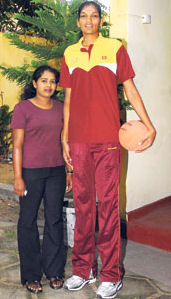
\includegraphics[height=2cm]{../images/Dharshani.jpg}
\end{center}

\end{frame}

\begin{frame}[fragile]\frametitle{}

\begin{alertblock}{Have a go}
Madison Robinson is the shortest Australian International player. What percentage of Australian women are between Madison and Dharshani’s heights?

\href{https://en.wikipedia.org/wiki/Madison Robinson}{\beamergotobutton{Madison}}

\end{alertblock}

\begin{knitrout}
\definecolor{shadecolor}{rgb}{0.969, 0.969, 0.969}\color{fgcolor}\begin{kframe}
\begin{alltt}
\hlcom{#Check your answer}
\hlstd{m}\hlkwb{=}\hlstd{(}\hlnum{168} \hlopt{-} \hlnum{161.8}\hlstd{)}\hlopt{/}\hlnum{6}
\hlkwd{pnorm}\hlstd{(d)}\hlopt{-}\hlkwd{pnorm}\hlstd{(m)}
\end{alltt}
\begin{verbatim}
## [1] 0.150724
\end{verbatim}
\end{kframe}
\end{knitrout}

\end{frame}


\begin{frame}[fragile]\frametitle{}

\begin{alertblock}{Have a go}
If 60\% of Australian women are below a certain height, what is that height?
\end{alertblock}

\begin{knitrout}
\definecolor{shadecolor}{rgb}{0.969, 0.969, 0.969}\color{fgcolor}\begin{kframe}
\begin{alltt}
\hlcom{#Check your answer}
\hlkwd{qnorm}\hlstd{(}\hlnum{0.6}\hlstd{,}\hlnum{161.8}\hlstd{,}\hlnum{6}\hlstd{)}
\end{alltt}
\begin{verbatim}
## [1] 163.3201
\end{verbatim}
\end{kframe}
\end{knitrout}
\end{frame}

\begin{frame}[fragile]\frametitle{}

\begin{alertblock}{Have a go}
If $X \sim N(8,16)$ find $P(X \leq 20)$.

\end{alertblock}

\begin{knitrout}
\definecolor{shadecolor}{rgb}{0.969, 0.969, 0.969}\color{fgcolor}\begin{kframe}
\begin{alltt}
\hlcom{#Check your answer}
\hlkwd{pnorm}\hlstd{(}\hlnum{20}\hlstd{,}\hlnum{8}\hlstd{,}\hlnum{4}\hlstd{)}
\end{alltt}
\begin{verbatim}
## [1] 0.9986501
\end{verbatim}
\begin{alltt}
\hlkwd{pnorm}\hlstd{(}\hlnum{3}\hlstd{)}
\end{alltt}
\begin{verbatim}
## [1] 0.9986501
\end{verbatim}
\end{kframe}
\end{knitrout}

\end{frame}


\begin{frame}[fragile]\frametitle{}

\begin{alertblock}{Have a go}
Given Australian male heights can be approximated by $X \sim N(175.6,7^2)$, what proportion of Australian man are similar height to Sydney superstar Adam Goodes (191cm) or West Coastruckman Nick Naitanui (201cm)?

\end{alertblock}

\begin{knitrout}
\definecolor{shadecolor}{rgb}{0.969, 0.969, 0.969}\color{fgcolor}\begin{kframe}
\begin{alltt}
\hlcom{#Check your answer}
\hlstd{a} \hlkwb{=} \hlstd{(}\hlnum{191}\hlopt{-}\hlnum{175.6}\hlstd{)}\hlopt{/}\hlnum{7}
\hlnum{1}\hlopt{-} \hlkwd{pnorm}\hlstd{(a)}
\end{alltt}
\begin{verbatim}
## [1] 0.01390345
\end{verbatim}
\begin{alltt}
\hlstd{n} \hlkwb{=} \hlstd{(}\hlnum{201}\hlopt{-}\hlnum{175.6}\hlstd{)}\hlopt{/}\hlnum{7}
\hlnum{1}\hlopt{-} \hlkwd{pnorm}\hlstd{(n)}
\end{alltt}
\begin{verbatim}
## [1] 0.000142497
\end{verbatim}
\end{kframe}
\end{knitrout}
\end{frame}

\end{document}
